\begin{frame}
\frametitle{Обучение с подкреплением}
\begin{columns}
\column{0.4\linewidth}
  \centering
  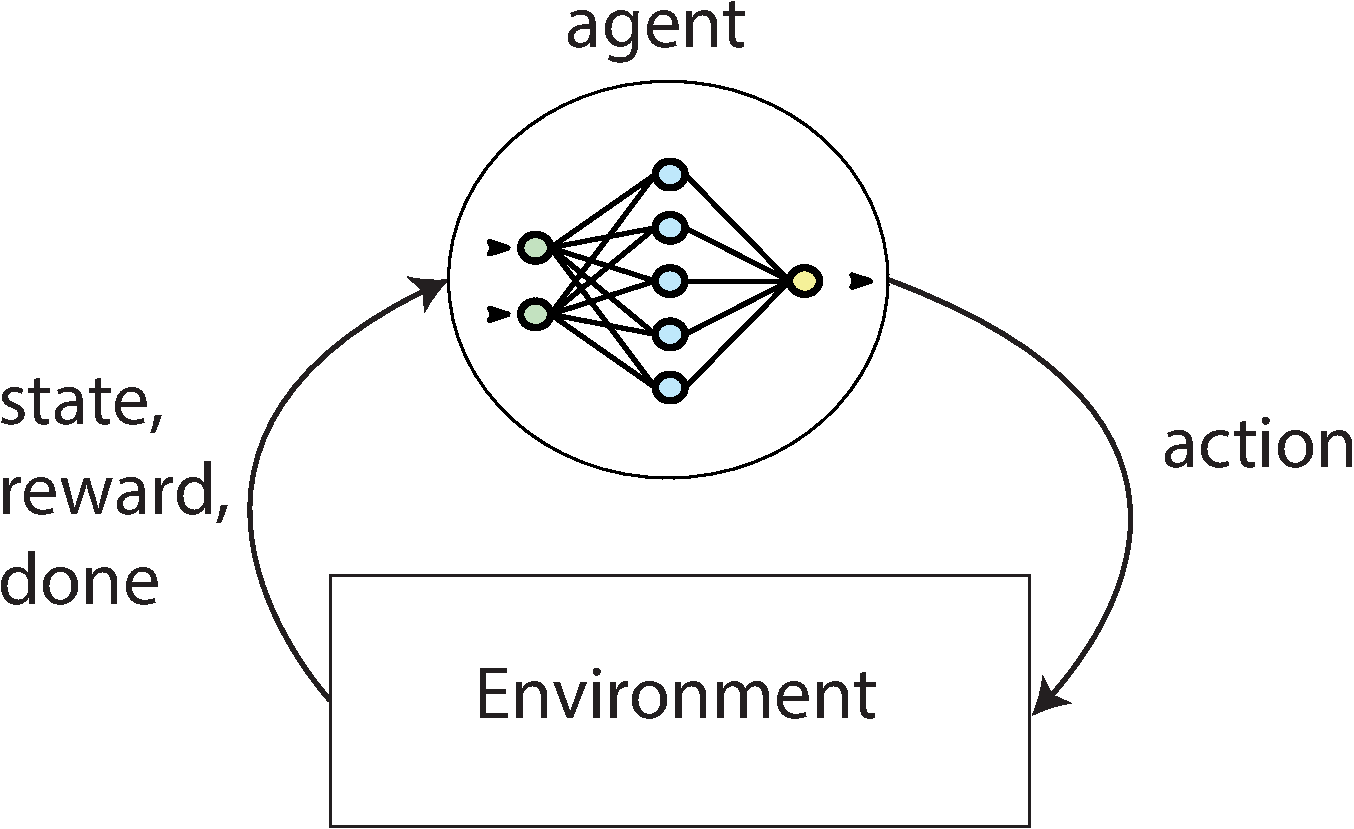
\includegraphics[width=1\linewidth]{images/rl_setting.pdf}
  
  \begin{equation*}
    <\mathcal{S, A, R, P}, \gamma>
  \end{equation*}

\column{0.6\linewidth}


\begin{align*}
& \ex_{\tau \sim \pi_{\theta}} [J(\tau)] = \ex_{\tau \sim \pi_{\theta}} \left[r_0 + \gamma r_{1} + \gamma ^ 2 r_{2} + ...\right] \\
& V(s_t) = \ex\left[\sum \gamma ^t r_{t}\right] \\
& Q(s_t, a_t) = \ex\left[r_t + \sum \gamma ^{t + 1} r_{t + 1}\right] \\
\end{align*}
\end{columns} 
\end{frame}

\section{Настройка оптического интерферометра методами машинного обучения с подкреплением}

\subsection{Постановка задачи}

\begin{frame}
\frametitle{Физические принципы работы и модель оптического интерферометра}
\begin{columns}
\column{0.5\linewidth}
  \centering
  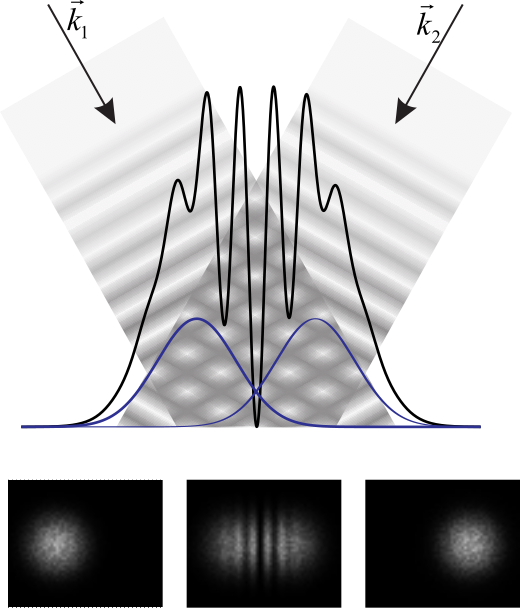
\includegraphics[width=0.9\linewidth]{images/interf_expl.png}

\column{0.5\linewidth}

\begin{align*}
& E(x,y,z)=\exp \left[-\frac{\left(x-x_{0}\right)^{2}+\left(y-y_{0}\right)^{2}}{r^{2}(z)}\right] \cdot \\
& \hspace{20pt} \exp \left[-i\left(k_{x} x+k_{y} y+k_{z} z + k\frac{x^2+y^2}{2\rho^2(z)} z\right)\right] \\
& E(x, y, z) = E_1(x, y, z) + E_2(x, y, z) \\
& I(x, y, z) = |E(x, y, z)|^2 = E(x,y,z) \cdot E^*(x,y,z) \\
& I= I_1 + I_2 + 2 \sqrt{I_1I_2}\cos(\Delta \phi)
\end{align*}

\end{columns} 
\end{frame}

\begin{frame}
\frametitle{Интерферометр Маха-Цендера}
  \centering
  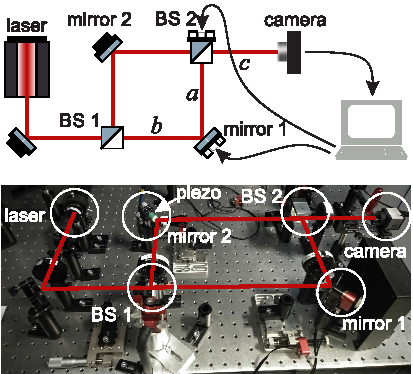
\includegraphics[width=0.8\linewidth]{scheme_with_experiment.pdf}
\end{frame}


\begin{frame}
\frametitle{Математическая модель интерферометра Маха-Цендера}
\begin{columns}
\column{0.6\linewidth}
  \centering
  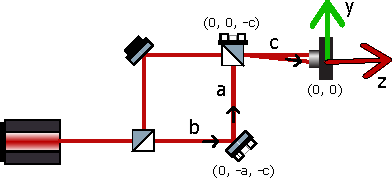
\includegraphics[width=1\linewidth]{images/MZI_matmodel.pdf}
  \begin{itemize}
    \item управление положением луча на камере $(x_0, y_0)$
    \item управление направлением $\vec{k}$
  \end{itemize}

\column{0.5\linewidth}
\begin{table} [htbp]
    \centering
    \begin{threeparttable}
        \begin{tabular}{| p{2.5cm} || p{2cm} |}
            \hline
            \hline
            параметр & значение \\
            \hline
            Mirror 2 $\to$ BS 2 & 200 mm\\
            BS 1 $\to$ Mirror 2 & 300 mm\\
            BS 2 $\to$ Camera & 100 mm\\
            radius & 0.95\\
            $\alpha_{{\mathrm{max}}(x,1)}$ & $5.2 \cdot 10^{-3}$ rad\\
            $\alpha_{{\mathrm{max}}(y,1)}$ & $3.7 \cdot 10^{-3}$ rad\\
            $\alpha_{{\mathrm{max}}(x,2)}$ & $2.6 \cdot 10^{-3}$ rad\\
            $\alpha_{{\mathrm{max}}(y,2)}$ & $1.8 \cdot 10^{-3}$ rad\\
            \hline
            \hline
        \end{tabular}
    \end{threeparttable}
\end{table}

\end{columns} 
\end{frame}


\begin{frame}
\frametitle{Видность интерференционной картины}

\begin{columns}
\column{0.4\linewidth}
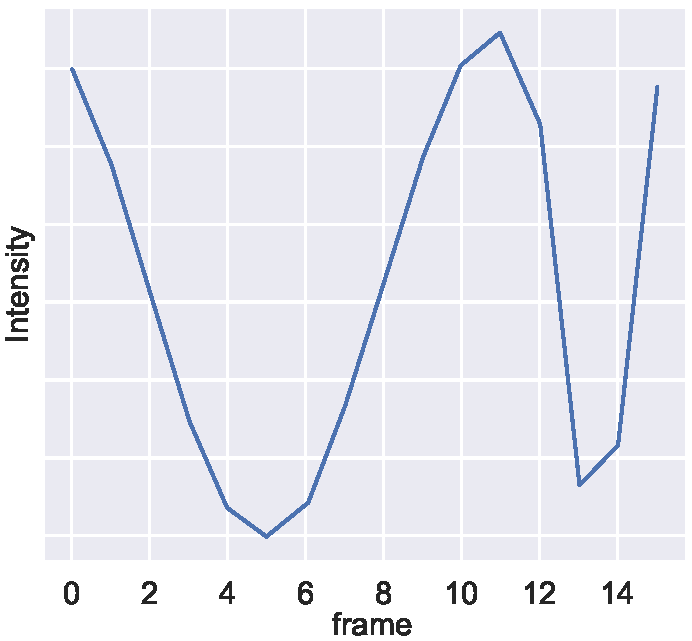
\includegraphics[width=1\linewidth]{itotal.pdf}

\column{0.5\linewidth}
\begin{align*}
& I(x,y,t)=|E_1(x,y,0)+E_2(x,y,0)e^{i\phi_{\mathrm{piezo}}(t)}|^2 \\
& I_{\mathrm{tot}}(t) = \iint_{-\infty}^{+\infty} I(x, y, t) {\mathrm{d}}x{\mathrm{d}}y \\
& V = \frac{            
        \max_{t}(I_{\mathrm{tot}}) - \min_t(I_{\mathrm{tot}})}
        {\max_{t}(I_{\mathrm{tot}}) + \min_t(I_{\mathrm{tot}})} \\
& V = \exp\left(- \frac{x_0^2 + y_0^2}{2 r^2}\right)  \exp\left[- \frac{(k_x^2 + k_y^2) r^2}{8}\right] \\
\end{align*}

\end{columns}
\end{frame}

\begin{frame}
\frametitle{Примеры интерференционных картин полученные в симуляции}
\begin{columns}
\column{0.7\linewidth}
  \centering
   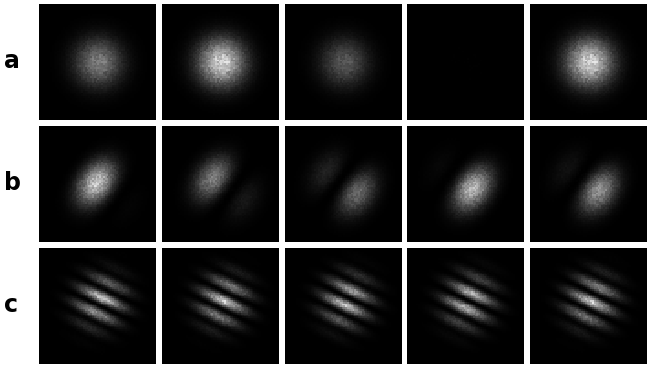
\includegraphics[scale=0.4]{images/visib_expl.png}

\column{0.5\linewidth}
\begin{description}
    \item V = 1
    \vspace{30pt}
    \item V = 0.3
    \vspace{30pt}
    \item V = 0.0026
\end{description}

\end{columns} 
\end{frame}


\begin{frame}
\frametitle{Математическая модель интерферометра Маха-Цендера с линзами}
\begin{columns}
\column{0.6\linewidth}
  \centering
   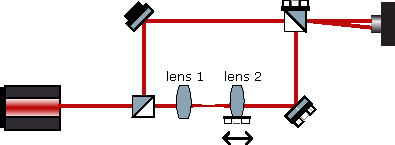
\includegraphics[width=1\linewidth]{images/MZI_expl_lenses.pdf}
  \begin{itemize}
    \item управление положением луча на камере $(x_0, y_0)$
    \item управление направлением $\vec{k}$
    \item \textcolor{red}{управление волновым фронтом}
  \end{itemize}

\column{0.5\linewidth}
\begin{table} [htbp]
    \centering
    \begin{threeparttable}
        \begin{tabular}{| p{2.5cm} || p{2cm} |}
            \hline
            \hline
            параметр & значение \\
            \hline
            BS 1 $\to$ Lens 1 & 50 mm\\
            $f_{\mathrm{lens 1}}$ = $f_{\mathrm{lens 2}}$ & 50 mm\\
            radius & 0.71 mm\\
            $\Delta_{\mathrm{max}}$ & 4.2 mm\\
            \hline
            \hline
        \end{tabular}
    \end{threeparttable}
\end{table}

\end{columns} 
\end{frame}

\begin{frame}
    \frametitle{Примеры интерференционных картин полученные на интерферометре Маха-Цендера с линзами}
    \centering
    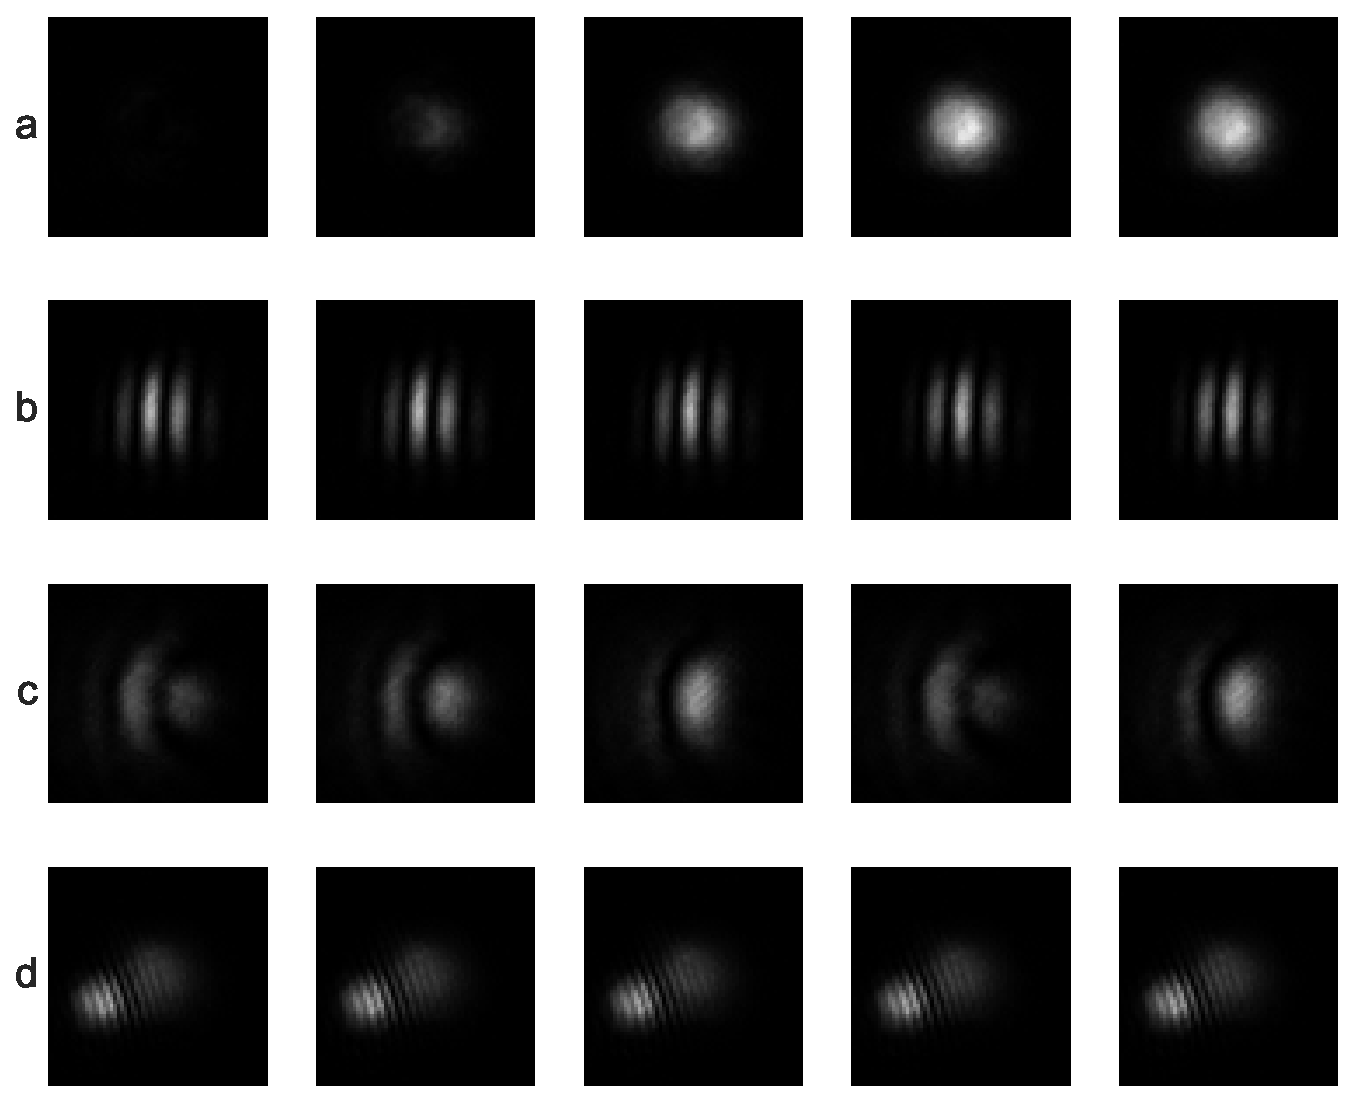
\includegraphics[width=0.8\linewidth]{images/Env_patterns.pdf}
\end{frame}

\begin{frame}
\frametitle{Видность интерференционной картины в интерферометре Маха-Цендера с линзами}
\begin{columns}
\column{0.3\linewidth}
\begin{align*}
& \dfrac{1}{q} = \dfrac{1}{\rho} - \dfrac{i \lambda}{\pi r^2} \\
& q^{\prime}=\dfrac{A q+B}{C q+D}\\
\end{align*}
\column{0.7\linewidth}
\begin{align*}
& \begin{bmatrix} A & B \\ C & D \end{bmatrix}=\begin{bmatrix} 1 & d \\ 0 & 1 \end{bmatrix} \hspace{25pt}\text{вакуум пространства длинны $d$}\\
& \begin{bmatrix} A & B \\ C & D \end{bmatrix}=\begin{bmatrix} 1 & 0 \\ -1/f & 1 \end{bmatrix} \hspace{5pt}\text{линза с фокусным расстоянием $f$} \\
& M = M_3^{ABCD} \times M_2^{ABCD} \times M_1^{ABCD}
\end{align*}
\end{columns}

\begin{equation*}
\begin{split}
    V =\frac{4}{\left(n^{2}+1\right) r_{\mathrm{u}}^{2}} \frac{1}{c} \exp \left(-\left(x_{0}^{2}+y_{0}^{2}\right)\left(\frac{1}{r_{\mathrm{u}}^{2} n^{2}}-\frac{n^{2}+1}{n^{6} r_{\mathrm{u}}^{6} c^{2}}\right)\right) \times \\ \times \exp \left(-\frac{n^{2}+1}{4 c^{2} n^{2} r_{\mathrm{u}}^{2}}\left(k_{x}^{2}+k_{y}^{2}\right)\right) \exp \left(\frac{\frac{\pi}{\lambda \rho^{\prime}}}{n^{2} r_{\mathrm{u}}^{2} c^{2}}\left(x_{0} k_{x}+y_{0} k_{y}\right)\right),
\end{split}
\end{equation*}
параметр $n=\dfrac{r_{\mathrm{l}}}{r_{\mathrm{u}}}$, $c^2 = (\dfrac{n^2 + 1}{n^2r^2_{\mathrm{u}}})^2$
\end{frame}

\begin{frame}{Численная модель интерферометра Маха-Цендера}
\begin{columns}
\column{0.5\linewidth}
\centering
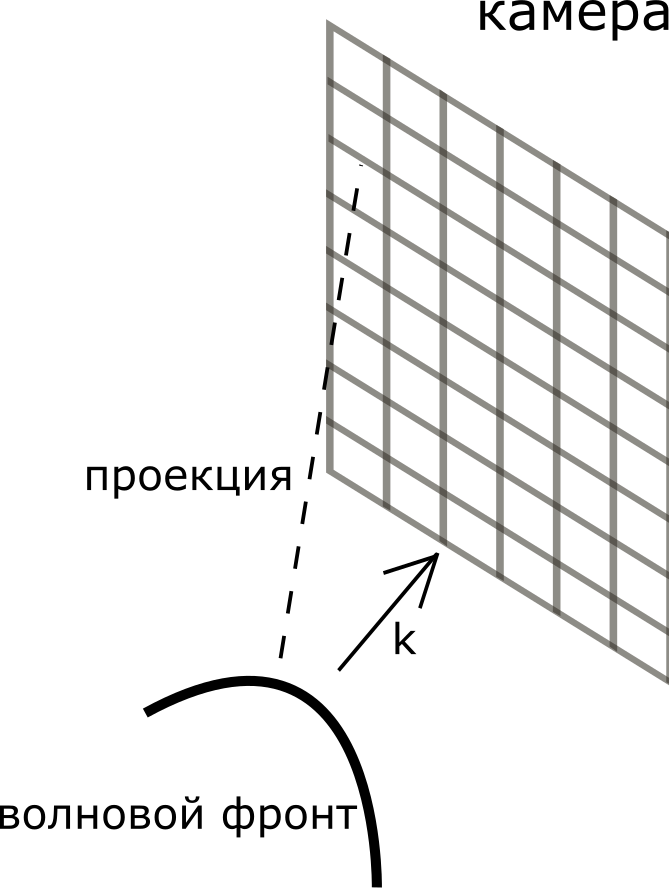
\includegraphics[width=0.8\linewidth]{images/wave_front_projection.png}
\column{0.5\linewidth}
\begin{enumerate}
    \item трассировка лучей 
    \begin{itemize}
        \item прохождение через зеркала $\vec{k}$, $(x_0, y_0)$
        \item радиус $r(z)$ и волновой фронт $\rho(z)$
    \end{itemize}
    \item вычисление интерференционной картины
    \begin{itemize}
        \item пространственное разрешение 64×64 пикселя
        \item временное разрешение 16 кадров
        \item параллельно для каждого пикселя и кадра
    \end{itemize}

    
\end{enumerate}

\end{columns}
\end{frame}

\subsection{Настройка с помощью DQN и TD3}


\begin{frame}{Настройка интерферометра с помощью алгоритма DQN}
\begin{columns}
\column{0.5\linewidth}
\centering
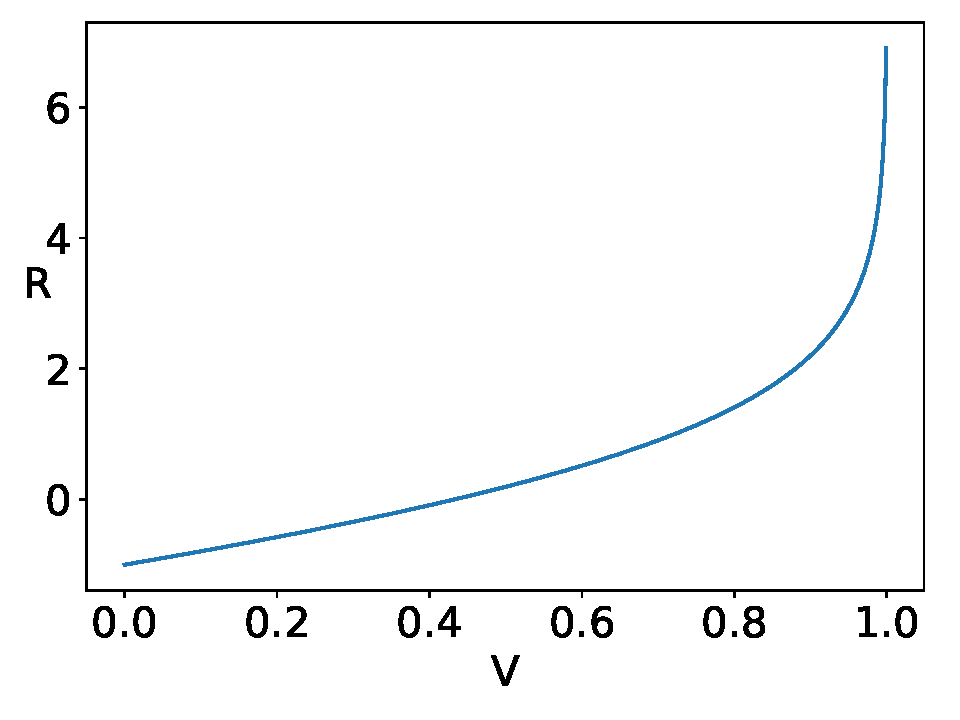
\includegraphics[width=1\linewidth]{images/reward_visib.pdf}
\column{0.5\linewidth}
\textbf{Награда}\\
$R = V - \log(1-V) - 1$\\
$V = 0.95 \to R = 2.9$\\
$V = 0.98 \to R = 3.9$\\
\textbf{Энкодер}\\
3-слойная сверточная  сеть [(32, 8, 4), (64, 4, 2), (64, 3, 1)] (Nature Mnih et.al, 2015)
\end{columns}
\vspace{10pt}
\textbf{Пространство наблюдений} 16 кадров 64x64 пикселя\\
\textbf{Пространство действий} \textcolor{red}{дискретное} (27/31) 
\textbf{Эпизод} 100 шагов, случайный reset $\pm \alpha_{\mathrm{max}}$, $\pm \Delta_{\mathrm{max}}$\\

\end{frame}

\begin{frame}{Настройка интерферометра с помощью алгоритма TD3}
\begin{columns}
\column{0.5\linewidth}
\centering
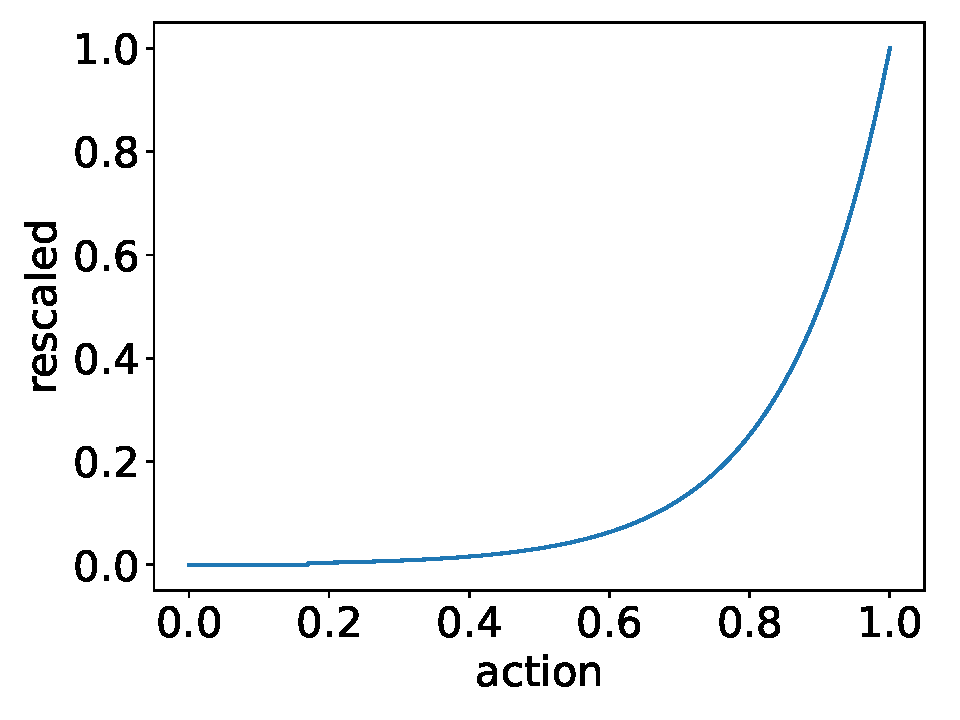
\includegraphics[width=1\linewidth]{images/rescale.pdf}
\column{0.5\linewidth}
\textbf{Награда}\\
$R = V - \log(1-V)$\\
\textbf{Масштабирование действий}\\
%{\setlength{\mathindent}{0cm}
\begin{equation*}
a^{\prime} =
   \begin{cases}
    {\mathrm{sign}}(a) \cdot 1000^{|a| - 1}  & \quad \text{если $|a_0| > 0.17$} 
    \\
    0  & \quad \text{иначе}
  \end{cases}
\end{equation*}%}
\textbf{Энкодер}\\
VGG-16
\end{columns}
\vspace{10pt}
\textbf{Пространство действий} \textcolor{red}{непрерывное} ($\mathcal{R}^4$/$\mathcal{R}^5$)

\end{frame}

\subsection{Программно-аппаратный комплекс Интерферобот}

\begin{frame}
    \frametitle{Программно-аппаратный комплекс Интерферобот}
    some text 4
\end{frame}

\begin{frame}
    \frametitle{Перенос из симуляции в реальность}
    some text 5
\end{frame}

\begin{frame}
    \frametitle{Настройки интерферометра Маха-Цендера без линз}
    some text 6
\end{frame}


\begin{frame}[allowframebreaks]
    \frametitle{Настройка интерферометра Маха-Цендера с системой линз}
    some text 7
    \framebreak
    some text mosdf
\end{frame}

\begin{frame}
    \frametitle{Выводы}
    some text 7
\end{frame}

% \subsection{Не нумерованные}

\section{Разработка алгоритма для игры NetHack с
применением машинного обучения с подкреплением}

\subsection{Декомпозиция игры NetHack на подзадачи}

\begin{frame}
\frametitle{NetHack challenge}
\begin{columns}
\column{0.6\linewidth}
  \centering
  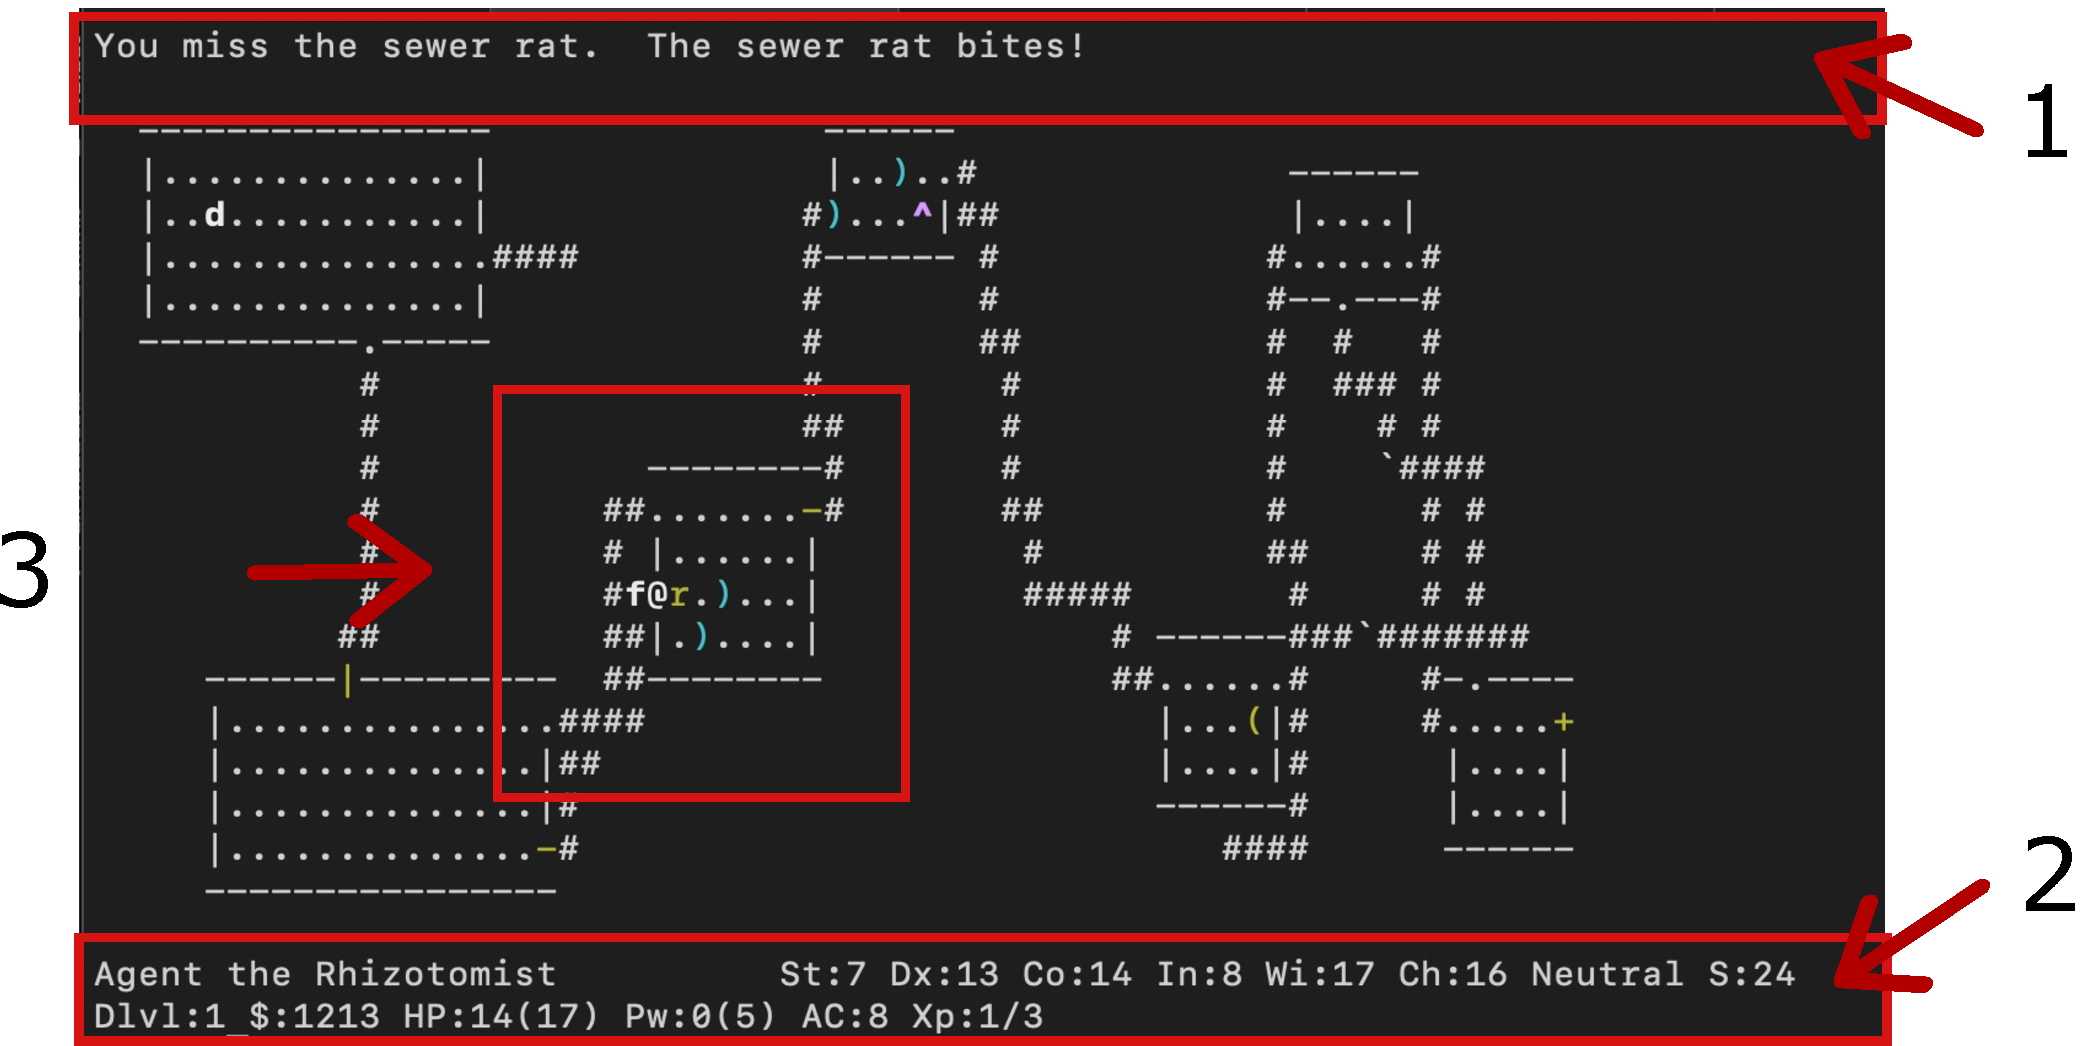
\includegraphics[width=1\linewidth]{images/nethack_map_view.pdf}
\column{0.55\linewidth}
\begin{enumerate}
    \item текстовое сообщение описывающее текущее событие
    \item статистика агента (здоровье, золото, сила, и др.) 
    \item окно центрированное возле текущего положения агента (@).
\end{enumerate}
\end{columns} 
\end{frame}


\begin{frame}
\frametitle{В чем ``challenge''?}
\begin{itemize}
    \item Процедурная генерация среды
    \item NetHack – очень длинная игра
    \item Много модальные наблюдения
\end{itemize}
\end{frame}


\begin{frame}
\frametitle{Декомпозиция игры NetHack на подзадачи}
    sometext
\end{frame}

\subsection{Объединение RL и алгоритмического подхода}

\begin{frame}
\frametitle{Обучение иерархического агента совмещающего обучение с подкреплением и алгоритмический подход}
    sometext 2
\end{frame}


\begin{frame}
\frametitle{Выводы}
    sometext 3
\end{frame}

%\begin{frame}
%    \frametitle{Изображения по-вертикали}
%    \centering
%    \vfill
%    \includegraphics[width=0.8\linewidth,height=0.1\textheight]{latex%} \\
%    \TeX
%    \vfill
%    \includegraphics[width=0.8\linewidth,height=0.2\textheight]{latex%} \\
%    \LaTeX
%    \vfill
%    \includegraphics[scale=0.2]{latex} \\
%    \vfill
%\end{frame}


%\begin{frame}
%    \frametitle{Изображения по-горизонтали}
%    \begin{minipage}[t]{0.47\linewidth}
%        \textbf{Составная \\ подпись 1}
%        \center{\includegraphics[width=1\linewidth]{knuth1}}
%    \end{minipage}
%    \hfill
%    \begin{minipage}[t]{0.47\linewidth}
%        \textbf{Составная \\ подпись 2}
%        \center{\includegraphics[width=1\linewidth]{knuth2}}
%    \end{minipage}
%\end{frame}


%\begin{frame}
%    \frametitle{Разделяющие линии}
%    \begin{minipage}[c]{0.47\linewidth}
%        \center{\includegraphics[width=1\linewidth]{latex}}
%        \bigskip
%        \hrule{}
%        \bigskip
%        \textbf{Составная \\ подпись 1}
%    \end{minipage}
%    \hfill
%    \vrule{}
%    \hfill
%    \begin{minipage}[c]{0.47\linewidth}
%        \flushright
%        \textbf{Составная \\ подпись 2}
%        \center{\includegraphics[width=1\linewidth]{knuth2}}
%    \end{minipage}
%\end{frame}

\section{Метод управления линейной и угловой скоростью шагающего робота основанный на обучении с подкреплением}

\begin{frame}
\frametitle{Постановка задачи управления шагающим роботом}
    sometext
\end{frame}

\begin{frame}
\frametitle{Метод управления линейной и угловой скоростью шагающего робота основанный на обучении с подкреплением}
    sometext 2
\end{frame}

\begin{frame}
\frametitle{Оценка результатов работы в симуляции}
    sometext 3
\end{frame}

\begin{frame}
\frametitle{Выводы}
    sometext 4
\end{frame}

%\begin{frame}
%    \frametitle{Четыре изображения}
%    \centering
%    \includegraphics[width=0.35\linewidth,angle=35]{latex}
%    \includegraphics[width=0.35\linewidth,angle=135]{latex}\\
%    \includegraphics[width=0.35\linewidth,angle=15]{latex}
%    \includegraphics[width=0.35\linewidth,angle=-15]{latex}
%\end{frame}

